\documentclass{UCF_ETD}
% \usepackage{times} % obsolete font package
\usepackage{url,hyperref,lineno,microtype,subcaption}
\usepackage{datetime, fmtcount, etoolbox, fcprefix}
\usepackage[T1]{fontenc}
\usepackage[utf8]{inputenc}
\usepackage{mathptmx}
\usepackage{graphicx}
\usepackage{amsmath,amssymb,amsfonts}
\usepackage{algorithmic}
\usepackage{textcomp}
\usepackage{cite}
\usepackage{graphics}
\usepackage{color,soul}
\usepackage{multirow,makecell}
% \usepackage[backend=biber,style=numeric]{biblatex}    
% %Use absolute paths to .bib-files for the subfiles to understand their location:
\usepackage{float}
\usepackage{chapterbib}
\usepackage{subfiles}
\newcommand{\ignore}[1]{}
\newcommand{\tss}[1]{\textsuperscript{#1}}
\renewcommand{\ul}{}


\title{\uppercase{Corticomuscular adaptation to mechanical perturbations in a seated locomotor task}} %Must be typed in all caps.
\author{\uppercase{Seyed Yahya Shirazi}} % typed in all caps



\prevdegreeii{B.Sc. AmirKabir University of Technology (Tehran Polytechnic), 2011}
\prevdegreei{M.Sc. AmirKabir University of Technology (Tehran Polytechnic), 2014}
% commands available for 
% \prevdegreei{ }
% \prevdegreeii{ }
% \prevdegreeiii{ }

\thesisname{dissertation}
% \thesisname prints out document type. Replace bracket text with dissertation for Ph.D students

\degreename{Doctor of Philosophy in Mechanical Engineering}
% type out degree name here.

\departmentsname{Mechanical and Aerospace Engineering}
% replace with department name if applicable.  Otherwise, do not include.

%\schoolname{Kenneth G. Dixon School of Accounting}
% replace with school name if applicable.  Otherwise, do not include.

\collegename{Engineering and Computer Science}
% replace with college name

\termname{Spring}
% replace with semester

\termyear{2021}
% replace with year. Term year is also used to generate copyright year.

\advisorname{Helen J. Huang}
% replace with Major Professor if applicable.  Otherwise, do not include.


\begin{document}

\frontmatter
% applies roman numerals as page numbers

\maketitle
% prints out school info as named above

\copyrightpage{~Seyed Yahya Shirazi}
% includes copyright symbol. Term year is automatically inserted before the author name.  Replace the author name with your own, but keep the tilde in place. 

\begin{abstract}
Seated locomotor tasks such as cycling or recumbent stepping improve walking performance during rehabilitation. Cortical control during walking is most pronounced when the person is perturbed. But, the electrocortical dynamics during perturbed seated tasks has not been studied in detail. The primary purpose of this research was to quantify cortical and muscular responses to mechanical perturbations during recumbent stepping. We also aimed to quantify possible differences between young and older adults' responses to perturbed stepping. Before 
% abstract files can be added here.  I recommend using \input over \include
\end{abstract}

\dedication{Dedicated to my love, Maryam.}
% creates vertically and horizontally centered dedication page.  If larger than a paragraph, remove the \vspace*fil commands from the dedication section in the class file.

\begin{acknowledgments}
The acknowledgments page is optional. If you choose to use it, it should appear after the Abstract, but before the Table of Contents.
\end{acknowledgments}

\tableofcontents

\listoffigures

\listoftables

\mainmatter
% restarts page numbering with arabic numbers

\subfileinclude{chapters/chap0}

\subfileinclude{chapters/chap1}

\subfileinclude{chapters/chap2}
% \begingroup
% % \renewcommand{\section}[2]{}%
% \renewcommand{\chapter}[2]{}% for other classes

% \endgroup



% If you choose to number headings and/or subheadings (e.g. 3.1, 3.1.1), you will need to change the secnumdepth to reflect the degree of numbering you wish to implement throughout your document.  

% This template is currently set to 0 so that chapter headings are numbered, but subheadings are unnumbered.

% Unless the nature of your ETD requires unique chapter headings such as creative MFA projects, set the secnumdepth to a minimum of 0 to insert chapter numbering.  

% To number subheadings, change the number to 5 to include all possible subheadings. 

% Creative works using chapter headings for a novel or other creative work will need to change the secnumdepth to -1 to remove the chapter name from the heading.

\chapter{FINDINGS}
Chapter Four, also called ``Results'' or ``Data Analysis,'' usually provides detailed findings of the research.  This chapter is where tables and figures most often appear, so make sure formatting is consistent.

\section{Sample Table}
The following sample table is an example of acceptable table formatting. Descriptive titles appear above tables and may appear either on one line or stacked and single-spaced. The table itself may also be single-spaced as necessary. If at all possible, try to keep tables and/or figures all on one page. If necessary, start the table or figure on a new page, even if this means leaving blank space on the preceding page. If you must split a table over multiple pages, repeat the table headings and continue. It is not necessary to repeat the table title.

% If tables or figures are being inserted in the middle of a sentence rather than at the end of the paragraph, change the place signifier to [h!] to override LaTeX's placement.

\begin{table}[h]
\centering
\caption{Classroom Tallies}
\begin{tabular}{ |c|c|c|c|}
\hline
D & A & B & C\\
\hline
E &  3  & 4 & 7\\
\hline
F  &  5   & 8 & 9\\
\hline
\end{tabular}
\end{table}

\section{Sample Figure}
The following is a sample figure with acceptable figure formatting. For figures, be sure you format both the figure and the figure title consistently. This includes placement (centered or left-justified), spacing before and after, line spacing, point size and font.

\begin{figure}
\begin{center}
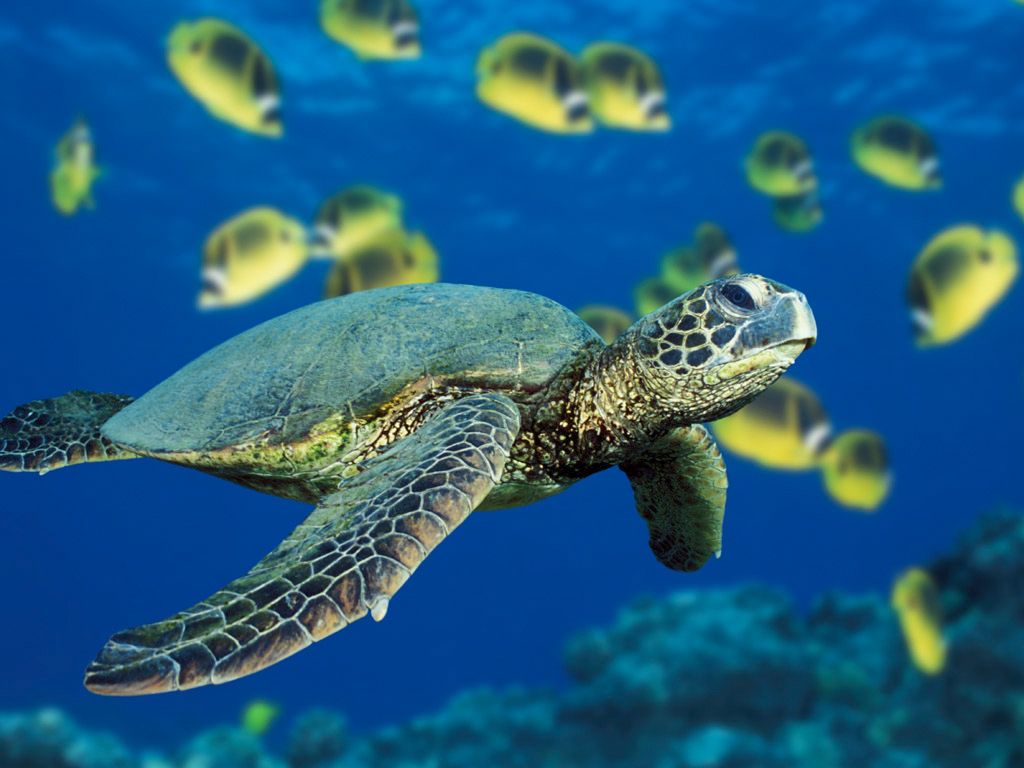
\includegraphics[scale=0.5]{Picture1}
\caption{Green Sea Turtle}
\end{center}
\end{figure}

\chapter{CONCLUSION}
Chapter Five, also called ``Summary,'' ``Conclusion,'' or ``Recommendations,'' usually presents a conclusion to the research, offers recommendations to the problem investigated, or discusses implications for future studies.

\section{Bookmarks}
A few words about bookmarks. Frontmatter entries, like the Abstract, Acknowledgments and the Table of Contents should appear in the bookmarks – but not in the Table of Contents. The TOC contains only pages that appear after the Table of Contents in the document, usually beginning with the List of Figures. So, bookmark and Table of Contents entries do vary.
However, bookmarks should include all major and chapter headings and at least first-level subheadings EXACTLY as they appear in the document (and the TOC). And readers should be able to link to pages within the ETD from all of the bookmarks, the TOC entries, as well as the Lists of Figures and Tables.
% all bookmarks are created through hyperref, so be sure that any additional packages are compatible.

\appendix

\chapter{TITLE OF APPENDIX}
\newpage
% You must include a \newpage command after each appendix.  And each appendix can be inserted as a chapter after the \appendix command.  

% This template is set to auto-letter multiple appendices.  

% If you change the secnumdepth to -1  and use multiple appendices, you must include the appendix name with the appendix title, such as APPENDIX A: TITLE.  If you have only one appendix, title it APPENDIX: TITLE.

% If you use chapter numbering and have only one appendix, you will need to comment out line 753 in the class file, containing the command \gdef\thechapter{\@Alph\c@chapter}}, and uncomment line 754 to define \gdef\thechapter{}} and remove the auto-lettering.


\noindent\labelitemi{~Begin appendix text on the page following the buffer page by using the newpage command.}\\
\labelitemi{~Continue Arabic pagination; do not restart page numbering with an appendix}\\
\labelitemi{~Use the same style and format for buffer page headings as you do for other body chapter headings.}\\
\labelitemi{~Letter, don't number, appendixes (e.g. APPENDIX A, APPENDIX B, etc.)}\\
\labelitemi{~If you have only one appendix, do not letter it at all}\\
\labelitemi{~Appendixes should follow the margin and other formatting requirements from the rest of the document}\\


\chapter{SECOND APPENDIX}
\newpage

Supplementary documentation.

\backmatter

% \begin{thebibliography}{99}

% \bibitem{Turkle95}
% 	Sherry Turkle,
% 	\emph{Life on the Screen}.
% 	Cambridge, MA: MIT Press,
% 	1995.

% % this template does not include any packages for references.  It is compatible with natbib and other common reference packages, but you will need to add them to the document.
% \end{thebibliography}

\end{document}